\documentclass{article}
\usepackage{amsfonts, amsbsy, amssymb, amsmath, graphicx, float, subfigure, natbib}

\tolerance=5000 
\textwidth=16.6 cm 
\oddsidemargin=-.04 cm
\evensidemargin=-.04 cm 
\topmargin=-1.3 cm 
\textheight=22.9 cm




\newtheorem{definition}{Definition}
\newtheorem{assumption}{Assumption}
\newtheorem{hyp}{Hypothesis}
\newtheorem{theorem}{Theorem}
\newtheorem{lemma}{Lemma}[section]
\newtheorem{corollary}{Corollary}[section]
\newtheorem{proposition}{Proposition}[section]

\begin{document}

\bibliographystyle{natbib}










\section*{Index Two Saddle Example: A `'Global'' Dividing Surface}


The influence of index two saddle points on reaction dynamics has been studied in \cite{ezra2009phase,collins:244105,Haller10,Mauguiere13}. The construction of a dividing surface for general index $k$ saddles was given in \cite{collins:244105}.  However, in this section we describe a `'global dividing surface'' that is associated with an index two saddle point and two index one saddle points. Such a structure was constructed in analyzing the isomerization dynamics of a buckled nanobeam in \cite{collins2012isomerization}. Intriguingly, a similar geometrical structure arose on the study of the so-called ''roaming phenomenon'' in \cite{Harding_et_al_2012, suits14}. Consequently, this type of geometrical structure could be more widespread in reaction dynamics so we believe it may be useful to give an analytically tractable example of such a situation.

As opposed to our linear examples above,  for the system to have multiple saddle points it must be  nonlinear.  We will consider two identical uncoupled two well potential systems, as shown in Fig. \ref{fig:global DS 1}.

\begin{figure}[htb!]
\begin{center}
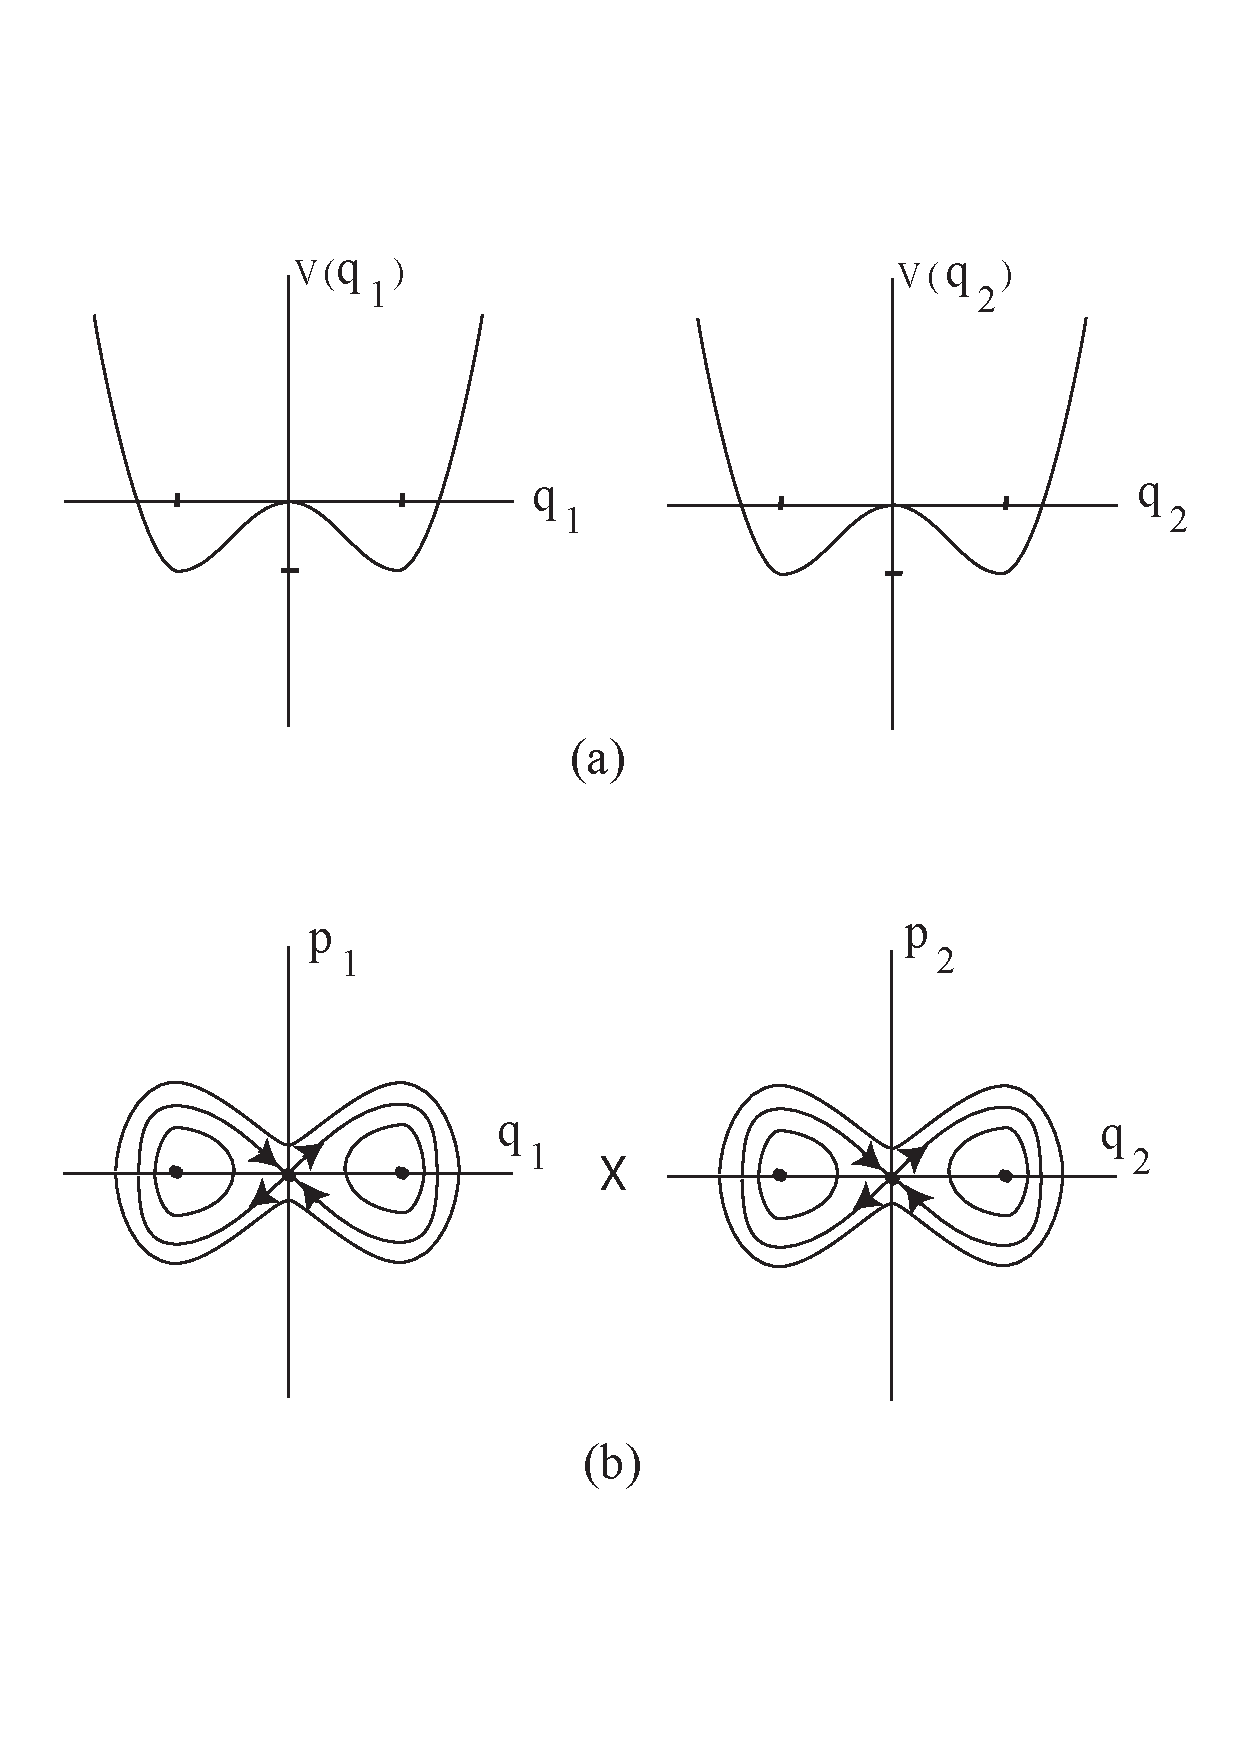
\includegraphics[width=10.0cm]{global_DS_1.pdf}
\end{center}
\caption{a) Graphs of the potential energy for the two uncoupled two well systems. b) Phase portraits for the two uncoupled two well systems.}
\label{fig:global DS 1}
\end{figure}

The Hamiltonian for this system is given by:

\begin{equation}
H =\underbrace{\frac{p_1^2}{2} - \frac{q_1^2}{2} + \frac{q_1^4}{4}}_{H_1} +
\underbrace{\frac{p_2^2}{2} - \frac{q_2^2}{2} + \frac{q_2^4}{4}}_{H_2},
\label{hamGDS}
\end{equation}


\noindent
with the associated Hamiltonian vector field:


\begin{eqnarray}
\dot{q}_1 & = & \frac{\partial H}{\partial p_1}=  p_1, \nonumber \\
\dot{p}_1 & = & -\frac{\partial H}{\partial q_1}= q_1 - q_1^3, \nonumber \\
\dot{q}_2 & = & \frac{\partial H}{\partial p_2}=  p_2, \nonumber \\
\dot{p}_2 & = & -\frac{\partial H}{\partial q_2}=  q_2- q_2^3. 
\label{hameqGDS}
\end{eqnarray}

\noindent
The potential energy is given by:

\begin{equation}
V(q_1, q_2) =  - \frac{q_1^2}{2} + \frac{q_1^4}{4}- \frac{q_2^2}{2} + \frac{q_2^4}{4}.
\label{pot}
\end{equation}

\noindent
The potential energy has nine critical points, which we list below, along with their stability type and total energy:

\begin{equation}
\begin{array}{cll}
(0,0), & \mbox{index two saddle}, & \mbox{total energy} \, \, 0,\\
(0,1), (0, -1), (1, 0), (-1, 0), & \mbox{index one saddles}, & \mbox{total energy} \, \,-{1}/{4} ,\\
(1, 1), (1, -1), (-1, 1), (-1, -1), & \mbox{minima}, & \mbox{total energy} \, \, -{1}/{2},
\end{array}
\end{equation}

\noindent
We illustrate the critical points of \eqref{pot} in Fig. \ref{fig:global DS 2}.

\begin{figure}[htb!]
\begin{center}
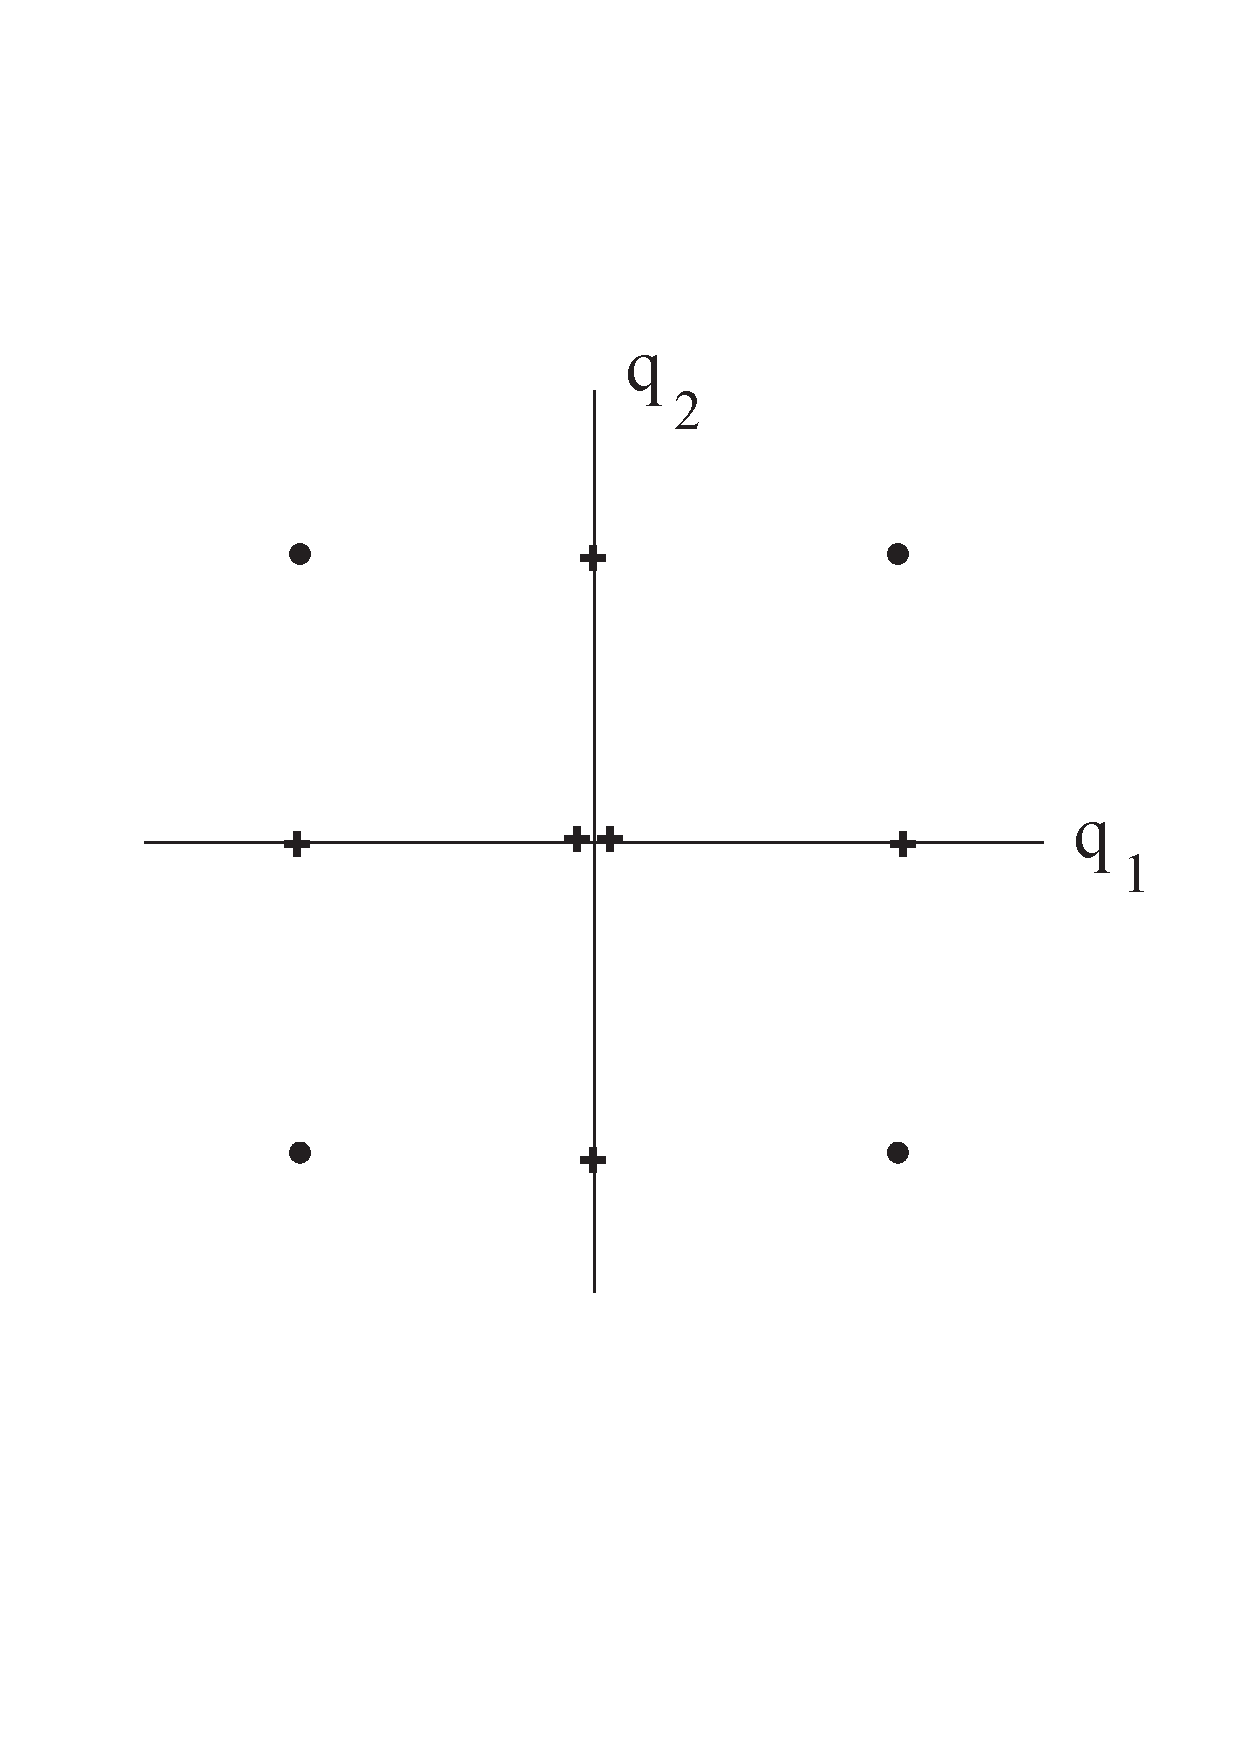
\includegraphics[width=10.0cm]{global_DS_2.pdf}
\end{center}
\caption{Critical points of \eqref{pot}. ++ denotes the index two saddle, + denotes index one saddles, and the black circles denote the minima.}
\label{fig:global DS 2}
\end{figure}

In order to consider a surface to be a dividing surface  we need to understand what the surface is dividing. In the language of chemical reactions,  index one saddles give rise to dividing surfaces that  divide reactants and products.  The examples above were designed  only to illustrate the geometry associated with the passage of trajectories through a dividing surface. In particular,  in the examples ``reactants'' corresponded to a region have a particular sign of the $q_1$  coordinate and `'products'' corresponded to a region corresponding to the opposite sign of the $q_1$ coordinate. and it was arbitrary which region was considered reactants and which products.  




For this example there are multiple wells, index one saddles, and one index two saddle. 
A natural  question to consider is how do the saddles influence  the motion of trajectories between the different wells? To some extent this question has been analyzed in \cite{collins:244105}. However, here  our goal will be only to construct a dividing surface that incorporates the index two saddle and two index one saddles, and to describe the role that these three saddles play in the dividing surface. Towards this end we consider the `'reaction problem'' of trajectories crossing $q_2=0$, but from a phase space perspective. 

The three dimensional energy surface is given by:

\begin{equation}
\frac{p_1^2}{2} - \frac{q_1^2}{2} + \frac{q_1^4}{4} +
\frac{p_2^2}{2} - \frac{q_2^2}{2} + \frac{q_2^4}{4}  = H_1 + H_2 = H,
\label{esGDS}
\end{equation}

\noindent
and a two dimensional DS separating trajectories with $q_2 <0$ from trajectories with $q_2 >0$ is given by:

\begin{equation}
\frac{p_1^2}{2} - \frac{q_1^2}{2} + \frac{q_1^4}{4} +
\frac{p_2^2}{2}  = H_1 + H_2 = H.
\label{GDS}
\end{equation}

\noindent 
The value of the total energy, $H$, plays a very important role in whether or not trajectories can cross this DS, as well as {\em how} they cross this DS.

Suppose we take:

\[
-1/4 < H_2 <0, \quad H_1 > 0.
\]

\noindent
In this case the $q_2$ component on a trajectory cannot change sign, but the $q_1$ component  can change sign.  This corresponds to crossing $q_2 =0$ by passing through one of the dividing surfaces corresponding to one of the index one saddles. As $H_2$ increases through zero, these two DSs merge, and now both the $q_1$ and the $q_2$ components of trajectories can change sign. In this way the index two saddle can be `'crossed''. A symbolic description of the different types of  trajectories classified  in terms of how they cross $q_2=0$ and their relation to the different saddles during the crossing is given in \cite{ezra2009phase,collins:244105}.

Finally, it is instructive to consider the word `'global'' in the phrase `'global dividing surface''. In this example there are two wells with $q_2 >0$ and two wells with $q_2 <0$. If one considers a reactive trajectory to be one that evolves from one well to another, typically one considers a dividing surface that only separates two wells. In this sense it is a `'local dividing surface''. However, in this example the dividing surface  is a boundary with multiple wells on each side of $q_2=0$. In order to give this configuration of wells, saddles, and global dividing surface meaning in a chemical reaction context, specific examples must be considered.  In this regard, the examples concerning with ``roaming reactions''  (see, e.g. \cite{Bowman2011Suits, bowman2011roaming}) discussed  in \cite{Shepler2011roaming, Harding_et_al_2012} are particularly interesting. They consider a global dividing surface that has the essential features of our example in that it is constructed from two index one saddles and an index two saddle at a higher energy than the index two. 








\bibliography{Ham_dyn.bib,roaming_v8.bib,reaction_dynamics.bib,rrkm_1.bib,vri_1.bib}


\end{document}


